\chapter{Pendahuluan}
\section{Latar Belakang}
Mengemudi merupakan salah satu pilihan bagi masyarakat untuk bepergian dari
suatu tempat ke tempat lain yang dituju. Contohnya adalah seorang wanita karir yang mengemudikan 
kendaraan pribadi dari rumah menuju kantor atau tempat kerjanya. Contoh lainnya adalah seorang sopir 
taksi yang mengemudikan kendaraannya untuk mengantar penumpang hingga sampai ke tujuan. Untuk dapat 
sampai ke titik tujuan, banyak rute yang dapat dilalui oleh seorang pengemudi. Seorang pengemudi, tentu 
saja akan mencari rute terdekat yang dapat dilalui, hal tersebut bertujuan untuk
menghemat penggunaan bahan bakar dan juga waktu. Pemilihan rute terdekat untuk dapat sampai 
ke tujuan menjadi cukup penting, karena saat ini mobilitas masyarakat yang semakin tinggi.
Aplikasi pencarian rute terdekat dapat membantu seorang pengemudi untuk menemukan rute terdekat 
untuk sampai ke tempat tujuan lebih cepat. Dengan cara menunjukkan rute menyetir terdekat dari satu 
tempat ke tempat lain. 

Aplikasi yang dibuat akan berbasis OpenStreetMap dan menggunakan 
algoritma Dijkstra. OpenStreetMap adalah portal peta terbuka yang menyediakan data dalam bentuk 
peta maupun XML, pengguna dapat mencari lokasi dan memilih area yang
diinginkan . Setelah pengguna memilih area yang diinginkan, pengguna dapat menggunakan
fitur export untuk mengunduh data XML pada area tersebut. Tampilan website
OpenStreetMap dapat dilihat pada Gambar \ref{fig:web_osm}.
\begin{figure}[h]
\centering
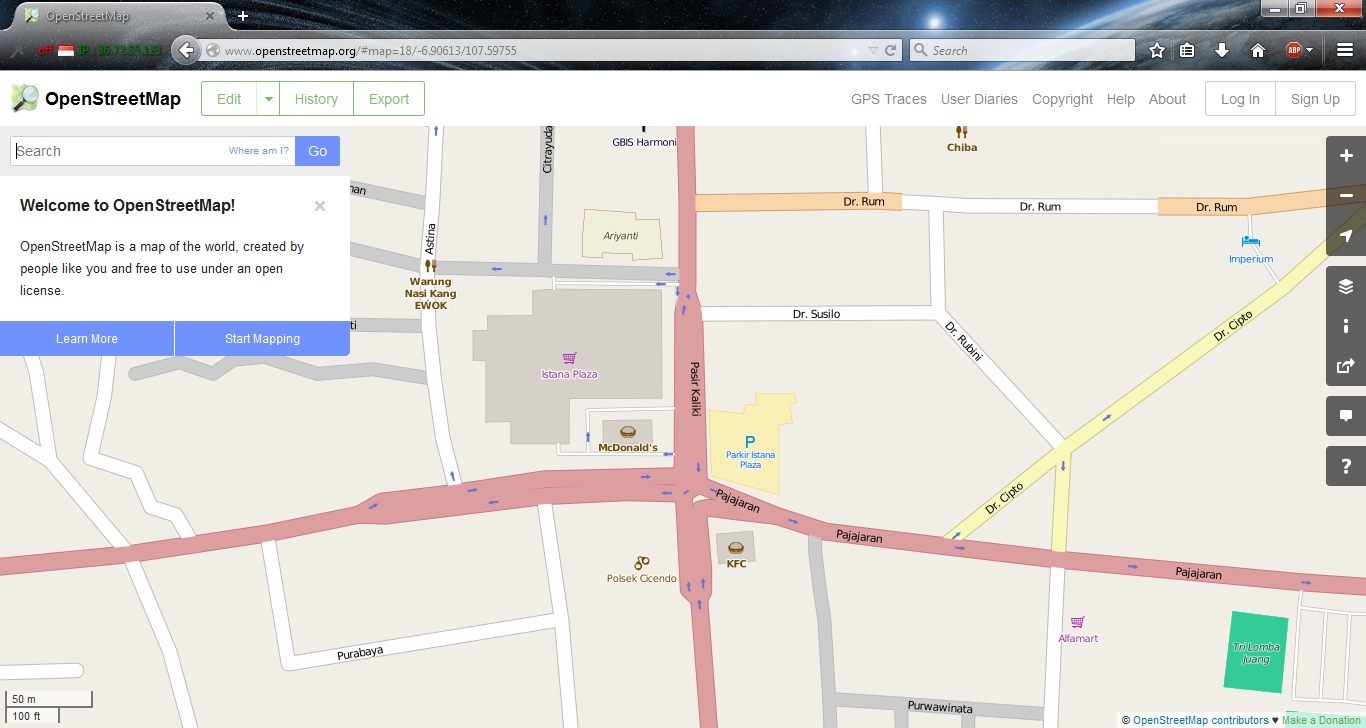
\includegraphics[scale=0.3]{Gambar/web_osm}
\caption[Tampilan website OpenStreetMap]{Tampilan website OpenStreetMap
\footnotemark[1]}
\label{fig:web_osm}
\end{figure}
\footnotetext[1]{http://www.openstreetmap.org}. Data yang
disediakan oleh OpenStreetMap dalam bentuk XML biasa disebut
dengan OpenStreetMap XML dan disingkat menjadi OSMXML. OSMXML adalah dokumen XML
yang berisi data-data peta OSM. Pada dasarnya, OSMXML berisi data primitif
(node, way, dan relation) yang merupakan arsitektur dari model OSM. Node
dapat diartikan sebagai titik pada peta dijital, way merupakan informasi garis
pada peta yang melambangkan jalan atau elemen lain seperti rel kereta, dan
relation memberikan informasi node-node yang bersinggungan, elemen
relation dapat menggambarkan suatu area seperti lapangan, taman bermain, rute
bus, dan lain-lain. Sedangkan algoritma Dijkstra
adalah algoritma untuk mencari jarak terpendek pada sebuah graf berarah dengan bobot yang bernilai tidak negatif pada setiap sisinya
\cite{Cormen:2001}. Graf adalah himpunan objek yang terdiri dari simpul(node)
dan sisi (edge), graf digambarkan sebagai kumpulan titik yang dihubungkan oleh garis. 
Contoh graf dapat dilihat pada Gambar \ref{fig:co_graf}.
\begin{figure}[h]
\centering
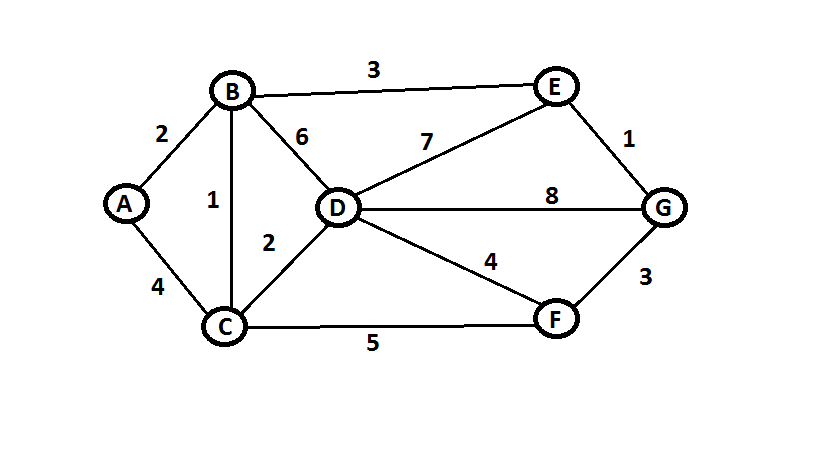
\includegraphics[scale=0.4]{Gambar/co_graf}
\caption[Contoh Graf]{Contoh Graf}
\label{fig:co_graf}
\end{figure}

Aplikasi yang dibuat akan mengolah data yang disediakan oleh OpenStreetMap dalam bentuk XML dan 
memodelkannya ke dalam bentuk graf. Selanjutnya akan digunakan algoritma Dijkstra untuk mencari 
rute terdekat pada graf tersebut dan menunjukkan hasilnya secara visual.

\section{Rumusan Masalah}
Berdasarkan latar belakang, maka rumusan masalah berikut: 
\begin{itemize}
	\item Bagaimana cara memodelkan data OSMXML menjadi sebuah graf?
	\item Bagaimana cara menggunakan atau mengimplementasikan algoritma Dijkstra
	pada sebuah graf untuk mencari rute terdekat?
	\item Bagaimana cara membuat visualisasi graf dan rute terdekat pada peta
	dijital?
\end{itemize}

\section{Tujuan}
Berdasarkan rumusan masalah yang telah diuraikan di atas, maka tujuan dari penelitian yang dilakukan
adalah:
\begin{itemize} 
	\item Mengetahui cara memodelkan data OSMXML menjadi sebuah	graf.
	\item Mempelajari cara kerja algoritma Dijkstra dan	mengimplementasikannya pada
	sebuah graf.
 	\item Mempelajari cara membuat visualisasi graf dan rute terdekat pada peta
 	dijital.
 \end{itemize}

\section{Batasan Masalah}
Batasan permasalahan dari pembuatan aplikasi ini adalah :
\begin{itemize}
	\item Aplikasi tidak mencari rute terdekat kedua dan seterusnya.
\end{itemize}

\section{Metodologi Penelitian}
Langkah-langkah yang akan dilakukan dalam melakukan penelitian adalah :
\begin{enumerate}
	\item Melakukan studi pustaka untuk mengetahui teori-teori yang dapat mendukung
	proses pembuatan aplikasi pencarian rute terdekat.
	\item Melakukan analisis teori-teori yang mendukung proses pembuatan aplikasi.
	\item Membuat rancangan aplikasi.
	\item Melakukan implementasi berdasarkan rancangan yang telah dibuat.
	\item Melakukan pengujian aplikasi.
	\item Melakukan pengambilan kesimpulan berdasarkan pengujian yang telah dilakukan.
\end{enumerate}

\section{Sistematika Pembahasan}
Pada setiap bab akan dibahas beberapa hal sebagai berikut :
\begin{enumerate}
	\item Bab Pendahuluan\\
	Bab 1 berisi latar belakang, rumusan masalah, tujuan, batasan masalah, metodologi penelitian, dan sistematika pembahasan.
	
	\item Bab Dasar Teori\\
	Bab 2 berisi teori-teori dasar mengenai OpenStreetMap, algoritma Dijkstra,
	Google Map Api, Graf, XML, dan beberapa teori lain yang mendukung pembuatan
	aplikasi.
	
	\item Bab Analisis\\
	Bab 3 berisi deskripsi sistem yang akan dibuat, analisis dasar teori, dan
	analisis cara kerja algoritma Dijkstra pada graf.
	
	\item Bab Perancangan\\
	Bab 4 berisi perancangan antarmuka aplikasi disertai beberapa gambar.
	
	\item Bab Implementasi dan Pengujian\\
	Bab 5 berisi hasil implementasi yang dilakukan disertai dokumentasi mengenai
	penjelasan aplikasi tersebut dan hasil pengujian yang dilakukan berupa
	\textit{screenshot}
	
	\item Bab Kesimpulan dan Saran\\
	Bab 6 berisi kesimpulan dari seluruh hasil penelitian dan saran untuk
	pengembangan aplikasi yang akan datang.
\end{enumerate}